
%*****************************************
\chapter{Discussion and Limitations}\label{ch:sixth}
%*****************************************

In this chapter, the main results of the study (see Chapter \ref{ch:fifth}) will be reviewed and analyzed, in relation to the recommendations proposed by Anonymous et al \cite{anonymous} (see Chapter \ref{ch:third}). Based on these results the universality of Anonymous et al.'s \cite{anonymous} approach will be discussed. Last, the limitations which were faced during the design and procedure of the study, will be presented.\\

Analogous to Anonymous et al., the main phases (orientation and input) were measured. In this study, an improved approach was taken towards enhancing the accuracy of the time measurements, specifically those of orientation time. Thus one of the limitations in Anonymous et al.'s \cite{anonymous} study, was that the quantitatively measured orientation times were not completely accurate. The concept FiPa was specially designed to implement Anonymous et al.'s \cite{anonymous} measurement method, to prevent this issue. \\
Based on a further recommendation by Anonymous et al. \cite{anonymous} the measurement of perceived efficiency was taken into consideration for the design of the study. Participants' perception of efficiency, regarding the ratios, was measured and assessed through a questionnaire. Participants were asked to directly compare the two main ratios "short/long" and "long/short" to each other, in terms of certain characteristics (mental effort, efficient, preference, longer input, longer search, etc.). 

Although the contrasting ratios "short/long" and "long/short" were designed to be symmetrical in terms of the phase lengths, quantitative results have shown that, on average, their length differed by 1176 ms, with "long/short" having the longest average duration (6056 ms). Nonetheless, apart the maximum orientation time of "long/short", the remaining times did not exceed 5202 ms. In reference to the orientation times of "short/long", this means that the "long phases" of both ratios did not differ substantially, and that in the worst-case there durations were in the same time range. The same is true for the maximum duration of the "short phases". short input ("long/short") and "short orientation" ("short/long") barely differed by 8ms. This shows that the design of the concept and the implementation of the ratios were suitable and successful for the purpose of this study, as in worst case they can be considered almost equally efficient in terms of their measured efficiency. \\

In terms of perceived efficiency, participants were first asked to evaluate the mental and practical tasks of each ratio, separately. They were asked to rate the annoyance of a ratio's orientation and the simplicity to memorize, as well as input its corresponding pattern. Surprisingly the memorization and input of the short pattern, as well as the long pattern, were considered easy to memorize and input, by all participants, on average. The difference between both ratios was notable regarding the annoyance of their orientation times. While, on average, all participants disagreed that "short orientation" was annoying, the average opinion regarding the annoyance of "long orientation" was neutral. Even if a strong \\




\textbf{Provide Efficient and Non-Interrupting Error Recovery}\\
As mentioned in Section \ref{4.3.2}, a form of \textit{error-recovery} was included into the application with the intention of enhancing its ease-of-use. Although the main focus of our study, was to solely examine certain ratios of \textit{orientation} and \textit{input phases}, it was indispensable to find out whether the \textit{error-recovery} feature had an impact on the measured and perceived \textit{orientation time}. For that, a question was added to the survey which only had to be answered if a participant encountered the \textit{error recovery} during the interaction. Answers were assessed through a Likert-scale (see figure \ref{fig:survey3}, question 19). Out of 19 participants, only 6 experienced the \textit{error recovery} (see figure \ref{fig:error})\footnote{We were able to obtain this information during the study, through the database view which was incorporated in the application (see figure \ref{fig:flow}) If a participant had more than three "search-fails", it meant that they encountered the \textit{error-recovery}}. When asked whether the pop-up window feature helped them find the pattern faster, five of the concerned participants agreed and only one disagreed. Moreover, half of the concerned participants (3) disagreed that the pop-up window elongated the searching process. However, one agreed and two answered did not notice any difference. Lastly, when asked whether they found the pop-up window annoying, four disagreed, one agreed, and another was indecisive (see figure \ref{fig:error}). In order to see whether \textit{error-recovery} had an impact on the concerned participants' performance, their quantitative data was examined. Luckily, they never encountered \textit{error-recovery} during the third level of each phase\footnote{As mentioned earlier, the first and second level of each phase in the application, were considered to an exercise. Only the third levels of each phase were involved in the quantitative evaluation.}, which meant that feature had no impact of the measured time. Nonetheless, the examination of the feature's effect still provided information on whether it's design was well accepted by participants. 

\begin{figure}[t!]
\centering
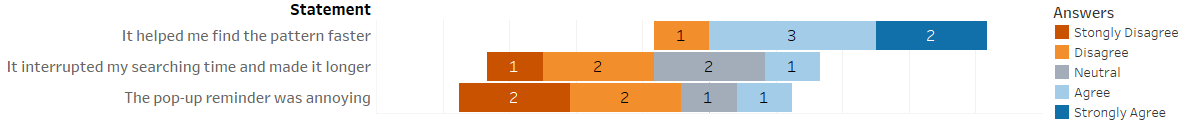
\includegraphics[width=15cm, height=3cm]{Chapters/graphics/ErrorRecovery.png}
\caption{A representation of how participants evaluated the \textit{error-recovery} feature of the application.}
\label{fig:error}
\end{figure}

\section{Limitations}

Although FIPA was designed to emulate an authentication process, to help participants adjust to the context of the study more easily, it is not clear whether their evaluation of the ratios might have differed if the they had interacted with them in real-life scenarios\footnote{Meaning if the participants had used the implementation of the concept as an authentication mechanism for a period of time (similar to the study design of Anonymous et al. \cite{anonymous}).}. As the concept was only used for a short period of time it was not possible to obtain a detailed conception on participants' preferences regarding the ratios.\\
Unfortunately, the study had to be conducted twice. The first study involved a wider and more versatile demographic, however, its quantitative results were not usable, by cause of an error in the implementation of the time measurements of the application. Sadly, the error was detected, afterwards, during the evaluation of the results. Consequently, an additional study had to be conducted and a new set of participants had to be recruited because the former participants were already familiar with the study and would have caused a bias in the results. The majority of the newly recruited participants were computer science students, as they had to be collected on short notice. This is another reason why the results of this study cannot be fully generalized, as the most of the participants had an IT-background and were also familiar with the importance of smartphone security. The outcome of the study would have been more interesting and convincing, if the participants had a wider demographic and did not use screen locks on their smartphone. In combination with a longitude study, it would have been possible to obtain more detailed information on the perceived efficiency and the user-acceptance of the main ratios, represented in the concept. As mentioned in Chapter \ref{ch:second}, the primary reason why smartphone users persist not to use screen locks is due to their inconvenience. It would have been interesting to find out, which of the ratios had the potential to motivate users to use authentication mechanisms on their smartphone and improve their smartphone security behaviour. Depending on their preference regarding the ratios it would have been possible to derive the true effect of orientation time and perceived efficiency. As a result a standard could be developed, based on the findings, to guarantee a better user-acceptance and higher perceived efficiency for future authentication concept propositions.

In the study, the questionnaire included a semantic differential, such that participants could evaluate the aesthetics of the application. The intention was to examine how participants perceived the aesthetics of the application and to see whether it had an influence on their performance in the test or their acceptance of the ratio. However, during the evaluation it was noted that these observations would exceed the scope of this thesis and distract from its true focus, namely the effect of orientation time on the perceived efficiency of authentication mechanisms.  
